\usetikzlibrary{calc,arrows.meta,patterns,angles,quotes}
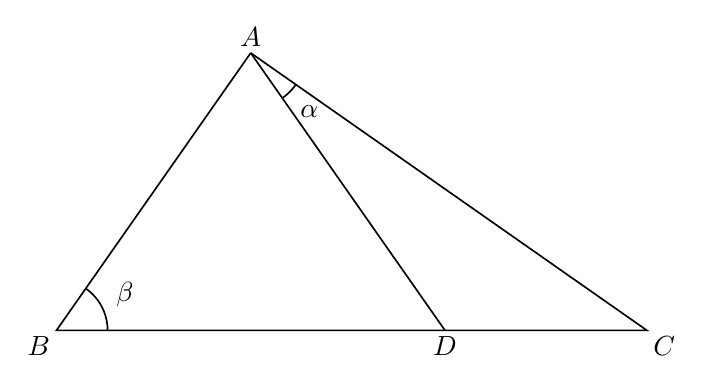
\begin{tikzpicture}[x=1cm,y=1cm,line width=.6pt,font=\normalsize,>=Stealth]
\coordinate (B) at (0.0000000000,0.0000000000);
\coordinate (C) at (7.5000000000,0.0000000000);
\coordinate (A) at (2.4674244625,3.5238473279);
\coordinate (D) at (4.9348489251,0.0000000000);
\draw (A)--(B)--(C)--(A);
\draw (A)--(D);
\node[above=2pt,inner sep=0pt] at (A) {$A$};
\node[below left=2pt,inner sep=0pt] at (B) {$B$};
\node[below right=2pt,inner sep=0pt] at (C) {$C$};
\node[below=2pt,inner sep=0pt] at (D) {$D$};
\draw (0.6500000000,0.0000000000) arc[start angle=0.0000000000,end angle=55.0000000000,radius=0.6500000000cm];
\draw (2.8689279680,2.9504408969) arc[start angle=-55.0000000000,end angle=-35.0000000000,radius=0.7000000000cm];
\node at (3.2098865828,2.7813852077) {$\alpha$};
\node at (0.8692706165,0.4525136410) {$\beta$};
\end{tikzpicture}
